\chapter{Fundamental Concepts}\label{ch:fundamental_concepts}
%%%%%%%%%%%%
%- Short introduction what we will go over.
%%%%%%%%%%%%
This chapter tries to condense some of the theoretic basics that will reoccur throughout the thesis. We start off with an introduction to the key aspects of X-ray free electron lasers including the more specific parts of self-seeding and X-ray pump -- X-ray probe techniques in section \ref{sec:xfel}. This is followed by a section about the formation of rare gas clusters and a particular emphasis on supersonic jets and pickup sources in section \ref{sec:cluster-theory}. We then dive into the interaction of light and matter, starting with X-ray scattering including the broad topic of phase retrieval in diffraction patterns in section \ref{sec:scattering-theory} and ending with the ionization of matter and formation of a nanoplasma.
\section{X-ray free electron laser}\label{sec:xfel}
%%%%%%%%%%%%
%- A historic introduction to FELs\\
%%%%%%%%%%%%
The advance of X-ray free electron laser in the recent years has enabled experimental ideas from long ago but has also opened entirely new branches to research \cite{Pellegrini-2016-RMP,Bostedt-2016-RMP}. So, let us start by investigating how that is. Thus far mostly synchrotron radiation facilities have provided X-rays to a great variety of scientific communities. In a synchrotron facility, a number of electron bunches is accelerated near the speed of light and then injected into a storage ring. Here, the electrons create an X-ray beam. The characteristics of this beam is called spectral brightness \cite{Mills-2005-IUCR} or sometimes brilliance\index{brilliance}. We can define the spectral brightness\index{spectral brightness} as \cite{Als-Nielson-2011-JWS}
\begin{equation}
B = \frac{n}{A\ \Theta\ t\ \Delta\! E},
\label{eq:spectral-brightness}
\end{equation}
with $n$ being the number of photons, $A$ the unit source size, $\Theta$ the divergence of the beam, $t$ the pulse duration and $\Delta\! E$ the spectral bandwidth of the light pulse. The spectral brightness is an overall measure of the quality of a light source. The development of modern synchrotron light sources is hence often measured and compared to previous achieved values. The motivation in the improvement of the spectral brightness is to let a sample interact with as many photons possible, in the shortest time as possible, with an energy resolution as best as possible. In other words, more brilliant light sources are needed to create images of even smaller particles, or look at dynamics that are even faster. To increase the spectral brightness drastically in the X-ray regime, one intended to build a laser alike X-ray source. 
\begin{figure}[t]
	\centering
		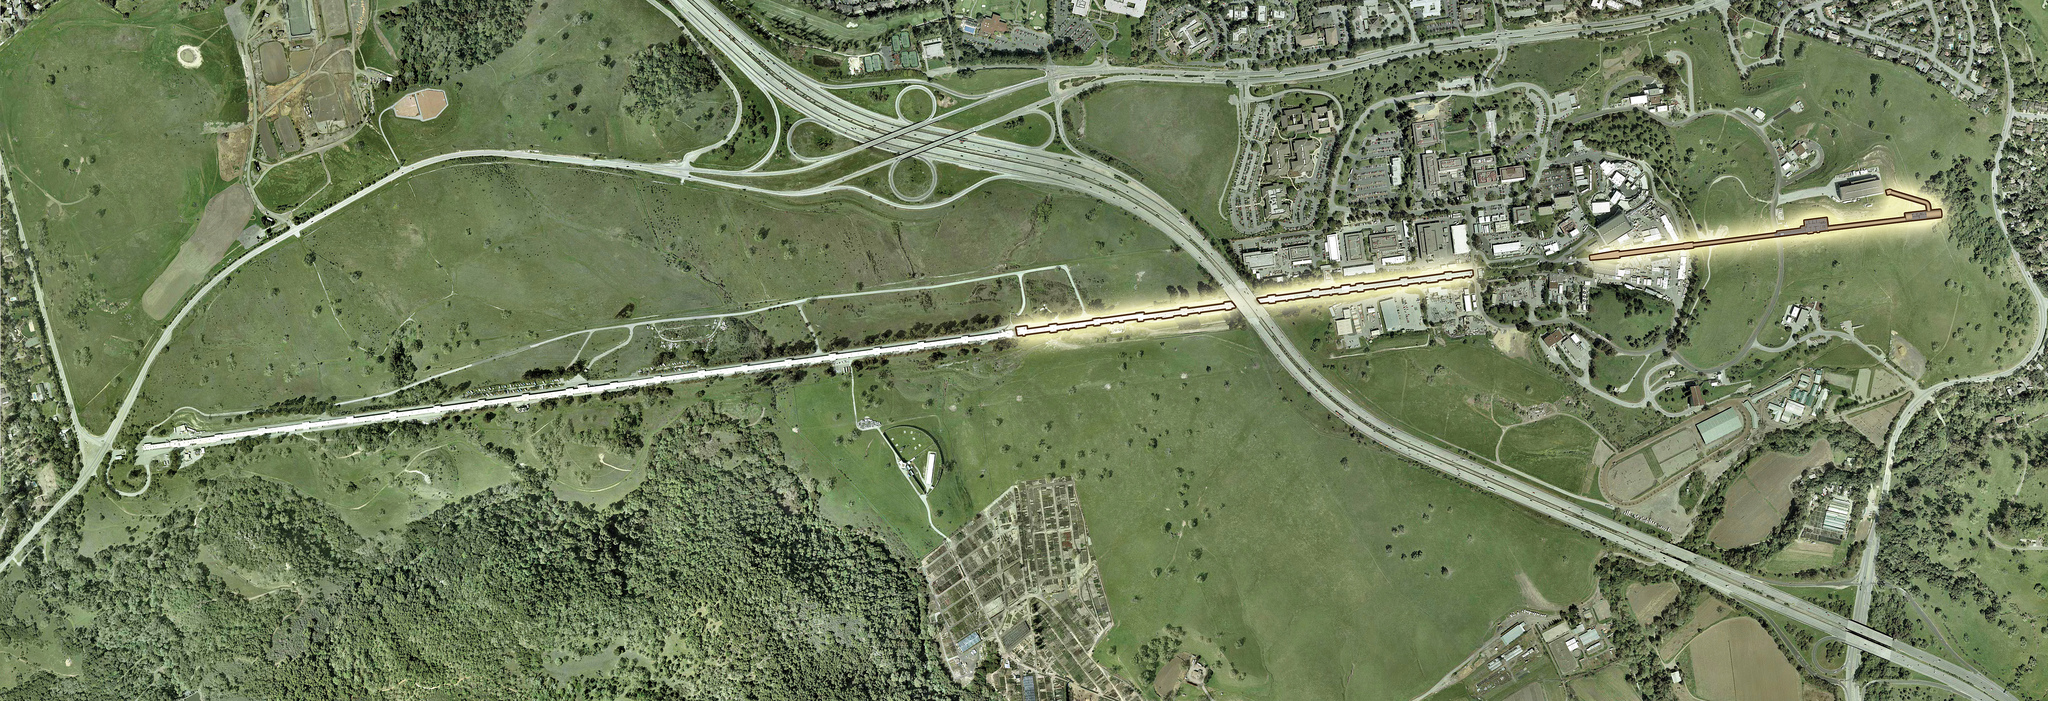
\includegraphics[width=1.00\textwidth]{images/aerial-view-lcls.jpg}
	\caption{Aerial view of the Linac Coherent Light Source\index{Linac Coherent Light Source} (LCLS). LCLS\index{LCLS|seealso {Linac Coherent Light Source}} uses the last third of the SLAC Linear Accelerator but is overall a ~4.1km long machine. The accelerator and buildings are stretched far because of the process light is generated. Image from \cite{SLAC-2009-Flickr}}
	\label{fig:aerial-view-lcls}
\end{figure}
To give a numerical example and to get a better understanding of the improvements needed, let us look at absorption dynamics in atoms and molecules. One can conservatively estimate that a typical cross section at soft X-rays (1 nm wavelength) is around $\sigma = 1$ megabarn (Mb) \cite{Bucksbaum-2011-Book}. Typical X-ray focii are round $A = 1 \mathrm{\mu m}^{2}$\footnote{Focus size at the AMO endstation at LCLS.} such that the number of photons needed $n_{in}$ to absorb just 1 photon per atom $n_{abs}$ can be calculated by
\begin{equation}
n_{in} = \frac{n_{abs} A}{\sigma} = \frac{10^{-8} \mathrm{cm}^{2}}{10^{-18} \mathrm{cm}^{2}}=10^{10} \mathrm{ photons}
\end{equation}
An example of a modern synchrotron source is NSLS-II and a rough estimate yields that it produces roughly $1.7 10^{4}$ photons per pulse in the Si111 bandwidth at pulse durations of a few ten picoseconds \cite{Williams-2016-PC}. That is far out of reach to investigate non-linear, or multi-photon, processes. While this back on the envelope type of calculation might be off by an order of magnitude or so depending on the specific case, it illustrates the order of magnitude improvement scientists were looking for. Unfortunately, synchrotron sources are not able to produce these conditions currently and regular optical laser methods can not easily be extended to also create X-rays. A United States defense program in the 80's wanted to use an X-ray beam as anti-(space)missile defense, where the X-ray beam was apparently generated through ignition of an atomic bomb \cite{Hecht-2008-OPN}. So, to reach the drastic higher number of photons per light pulse needed, it was proposed to build free electron laser \cite{Kondratenko-1980-PA,Bonifacio-1984-OC}. Free electron laser, amplify the light along a straight line to create laser alike radiation\footnote{The process to of the light create is explained in details in section \ref{sec:sase}.}. In the birds eye view of the Linac Coherent Light Source in figure \ref{fig:aerial-view-lcls}, one can imagine that it took several decades to build these kinds of sources. Today, free-electron lasers are able to increase the number of photons per pulse to currently $n_{in} = 10^{12}$ and achieve pulse lengths of a few femtoseconds. These are remarkable beam parameters and as a result LCLS was increasing the spectral brightness by many orders of magnitudes\footnote{See figure \ref{TBD} for an illustration of this improvement.}.
%While some applications are still under development \cite{Aquila-2015-StrucDyn,Weninger-2013-PRL}, free electron laser have made it possible to screen smaller protein crystals then previously possible to measure \cite{Chapman-2011-Nature} and are on track to study the thus far unknown protein structures \cite{Barends-2014-Nature}.
\subsection{Self amplification by spontaneous emission}\label{sec:sase}
%%%%%%%%%
%- Idea and schematic setup\\
%- Explain SASE including micro-bunching\\
%- Talk about the importance of monitoring the energy loss
%%%%%%%%%
\begin{figure}[t]
	\centering
		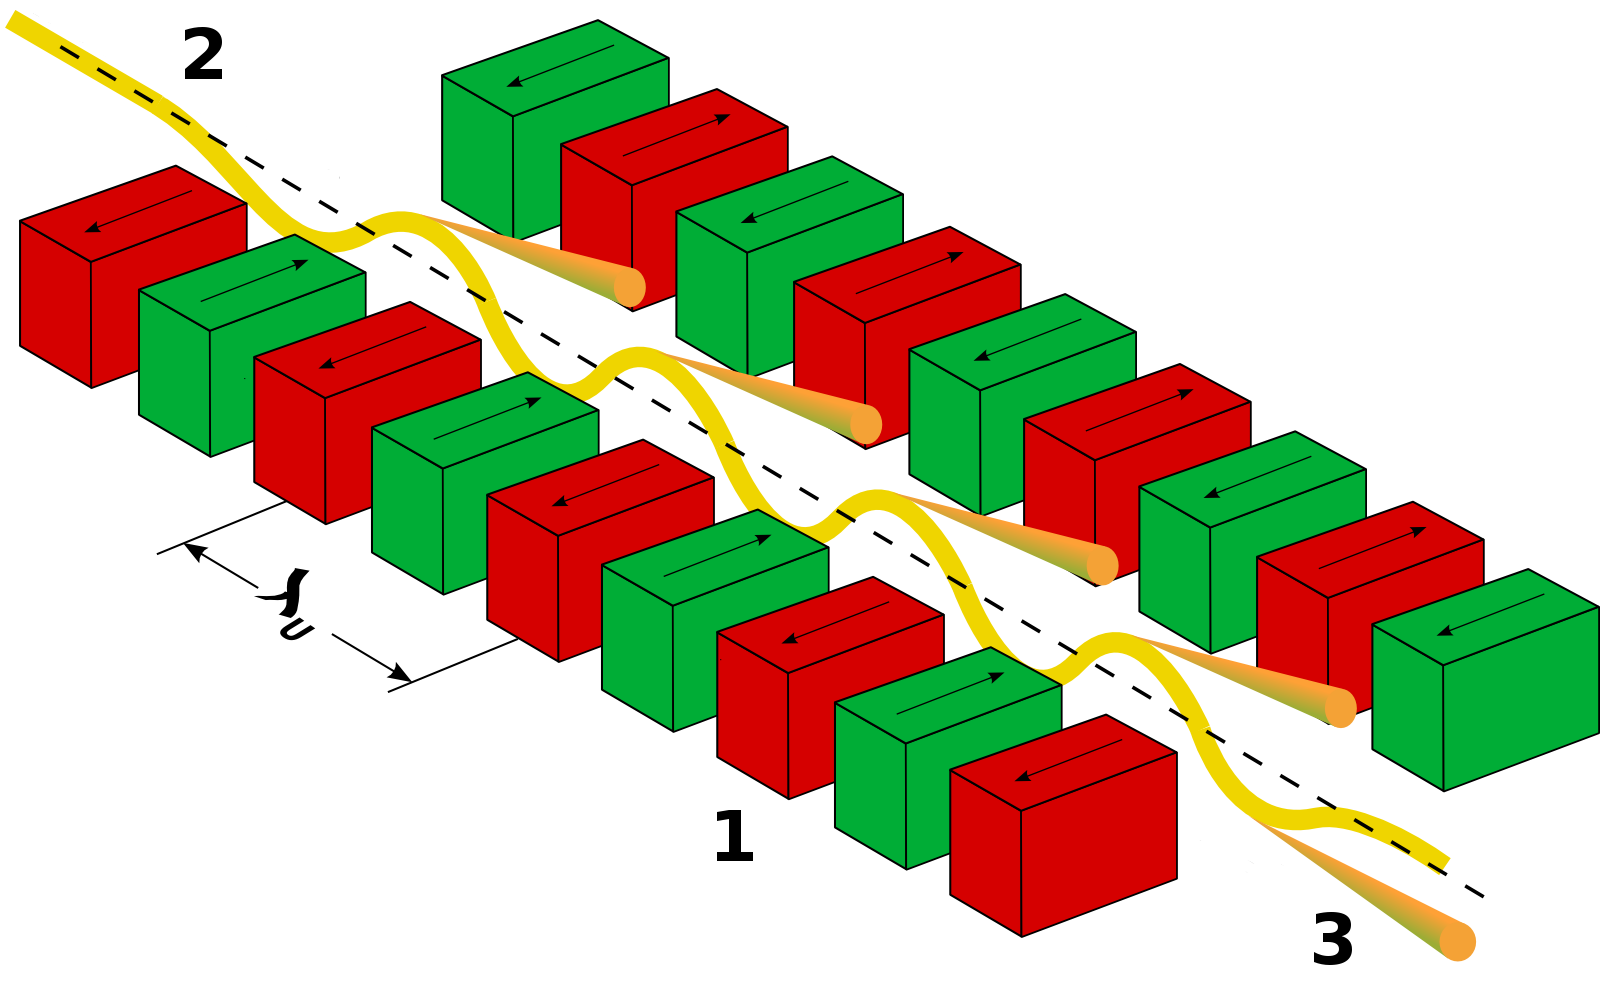
\includegraphics[width=1.00\textwidth]{images/Undulator.png}
	\caption{Schematic setup of an undulator with a period of $\lambda_{U}$. (1) Magnets in alternating polarity; the arrows indicate the direction of the magnetic field. (2) Incoming electron bunch near the speed of light. (3) Emitted light in beam direction due to sinusodial movement of the electron bunch. \cite{holst-2005-wiki}}
	\label{fig:undulator}
\end{figure}
In synchrotron lightsources as well as free electron lasers, X-rays are generated using wiggler and undulator magnets. In principle, an electron bunch is accelerated near the speed of light and then wiggled along its path using magnetic fields. The wiggeling causes the particles to emit radiation. Wigglers consist of magnets that are arranged in an alternating order to force the electron bunch on a sinusodial trajectory. In a Wiggler, the electrons emit a total power $P_{emitted}$ that is proportional to the number of magnets $m$. CITE
\begin{equation}
P_{emitted} \propto m,\quad \mathrm{in\ a\ wiggler\ magnet}
\end{equation}
The emitted radiation has a braod, continuous spectrum and the center of that spectrum can be controlled by changing the speed or kinetic energy of the electron bunch. Wigglers have been used at the Stanford Synchrotron Radiation Lightsource (SSRL) in 1979 to generate X-rays and were a great success. Continued development on the Wiggler design led to the idea of Undulators. A schematic setup of an undulator magnet can be seen in figure \ref{fig:undulator}. Wigglers and Undulators create radiation because of the same principle, an electron bunch is accelerated near the spead of light and then forced on a sinusodial pathway. In undulators, the separation of such magnets or undulator\index{undulator} period $\lambda_{U}$ and magnetic fields are chosen such that the emitted radiation per period constructively interferes with each other. The emitted wavelengths of undulators have a much more narrow pattern than thatof wigglers and because, strictly speaking, only one wavelength is amplified the emitted power $P_{W}$ now scales with CITE
\begin{equation}
P_{emitted}\propto m^{2},\quad \mathrm{in\ an\ undulator\ magnet}
\end{equation}
We can characterize an undulator by the undulator strength parameter $K$ and it is given by \citep{Huang-2007-PRSTAB}
\begin{align}
K &= \frac{e\ B\ \lambda_{U}}{2\ \pi\ m_{e}\ c}
\intertext{with the constants $e$ being the electron charge, $B$ being the magnetic field in the undulator, $m_{e}$ being the mass of an electron and $c$ being the speed of light, we can write}
K &\approx 9.34 10^{-3} B\ \lambda_{U}\ \mathrm{T\ m}UNIT CM?\label{eqn:undulator-strength}
\end{align}
Undulator magnets are large constructs of a few meters and their undulator period is on the order of centimeter. The electrons emit radiation in the nanometer wavelength regime because the electrons near the speed of light have to be considered relativistic and in the view of the electrons the undulator period $\lambda_{U}$ appears shorter. We can correct for the relativistic effects and express the main amplified wavelength $\lambda_{r}$ by CITE
\begin{equation}
\lambda_{r} = \frac{\lambda_{U}}{2 \gamma}\left(1+\frac{K}{2}+\gamma^{2}\Psi^{2}\right),\label{eqn:fundamental-wavelength}
\end{equation}
with the kinetic energy $\gamma$ of the electron beam in the undulator and $\Psi$ its observation angle. Equation \ref{eqn:undulator-strength} and \ref{eqn:fundamental-wavelength} also show that the wavelength in an undulator is determined by the undulator gap $\lambda_{U}$, the magnetic field $B$ in the undulator and the kinetic energy of the electron beam $\gamma$.\\
\begin{figure}
	\centering
		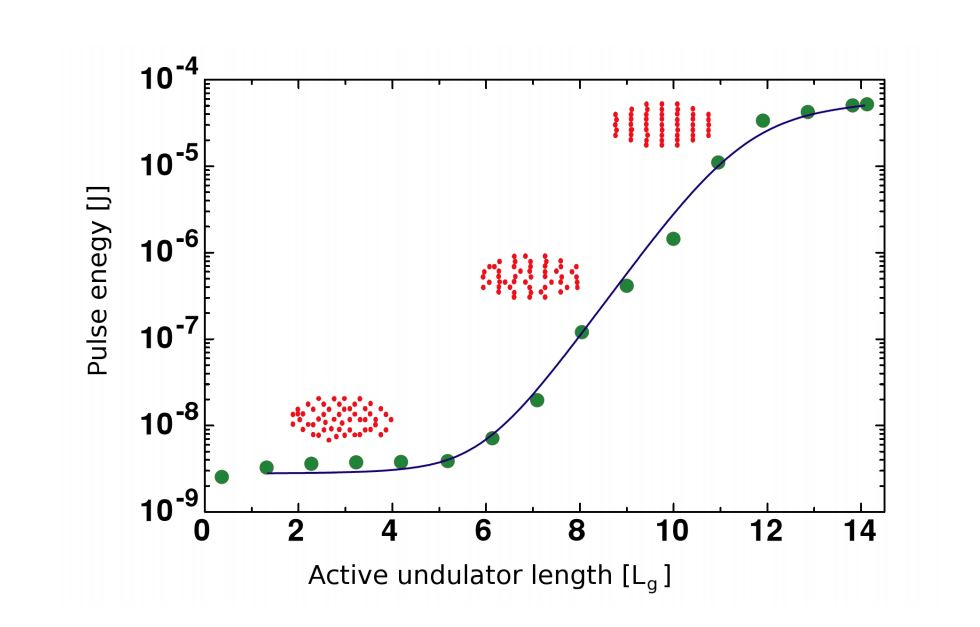
\includegraphics[width=1.00\textwidth]{images/gain-length.JPG}
	\caption{gain length. From \citep{Rupp-2013-Thesis,Rupp-2016-Springer}}
	\label{fig:gain-length}
\end{figure}
Undulators are also used in X-ray free electron lasers. The main difference to synchrotron radiation sources is that the light is amplified over a much longer straight line using multiple undulator magnets serially connected. LCLS has a 112m long undulator section. Over the course of this distance, microscopic effects start to play a role that could be neglected in typical synchrotron radiation sources. In vacuum, light will always be faster than electrons near the speed of light. This slight difference means that the copropagating photons and electrons have a phase difference and interact with each other. Depending on the phase, an electron will either gain or loose velocity. Over each undulator period, we can describe this \textit{slip} with $\lambda_{r}(\Psi = 0)$. As a result, the initial unifrom electron density in the electron bunch is peridoically modulated and the modulated electron bunch structure is called \textit{microbunching}. The creation of micobunching is illustrated in FIGURE. The increasingly structured electron beam amplifies a more narrow wavelength bandwidth and the number of electrons that are in phase with the photons increases over the travel length through the undulator. The electrons interact with the light field because of their narrow spatial and kinetic energy distributions. These parameters are characterized as the \textit{emittance} of an electron bunch. Only the linear accelerator of a FEL are able to compress the electron bunch in space and energy, i.e. create a low emittance electron bunch, such that it can interact with the photons as described above. The initial process that starts this light amplification is triggered by the first few photons that are spontaneous emitted and then subsequently amplified. Hence, this type of radiation (or FEL operation mode) is called \textit{Self Amplification by Spontaneous Emission} (SASE). It achieves laser alike amplification of the radiation power $P_{SASE}$ that scales with the number of electrons $N_{e}^{2}$
\begin{equation}
P_{SASE} \propto N_{e}^{2},\quad \mathrm{SASE\ operation}
\end{equation}
The characteristics of SASE radiation are its noisy and spiky photon spectrum, as seen in FIGURE, that come from the initial random (spontaneous) emission of photons.\\
X-ray free electron laser use one electron bunch and create one light pulse in a long set of undulator magnets, this is also called a \textit{single-pass high-gain} FEL. Due to the lack of optics, X-ray FEL operate in the high-gain mode. A X-ray FEL gain curve as a function of gain length $L_{g}$ can be seen in FIGURE. The electron bunch travels over a long distance in the undulators until it eventually reaches saturation. In saturation, the microbunching is most developed. Since the creation of X-rays is affected by the kinetic energy of the electron bunch $\gamma$ the electron bunch is not reused.
\subsection{Soft X-ray self seeding}
%%%%%%%%%%%%%%%%%%%%%%
%- Should I include this section? I could use it for the pump probe as well\\
%- Self seeding vs. seeded FELs\\
%- Schematic setup of a self seeding unit\\
%- Work towards self-seeded beams including spectrometer data
%%%%%%%%%%%%%%%%%%%%%%
\begin{figure}
	\centering
		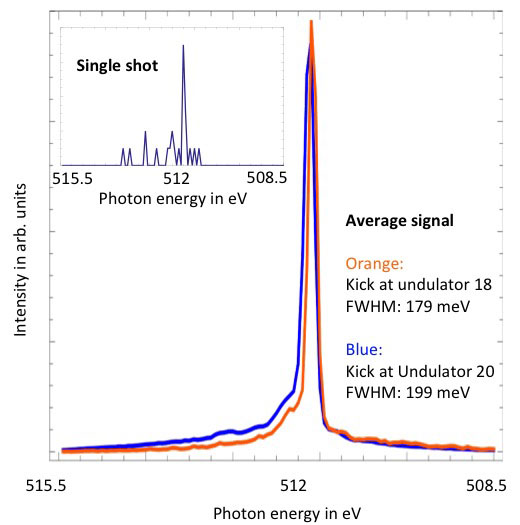
\includegraphics[width=0.49\textwidth]{images/Soft-X-ray-self-seeding.jpg}
		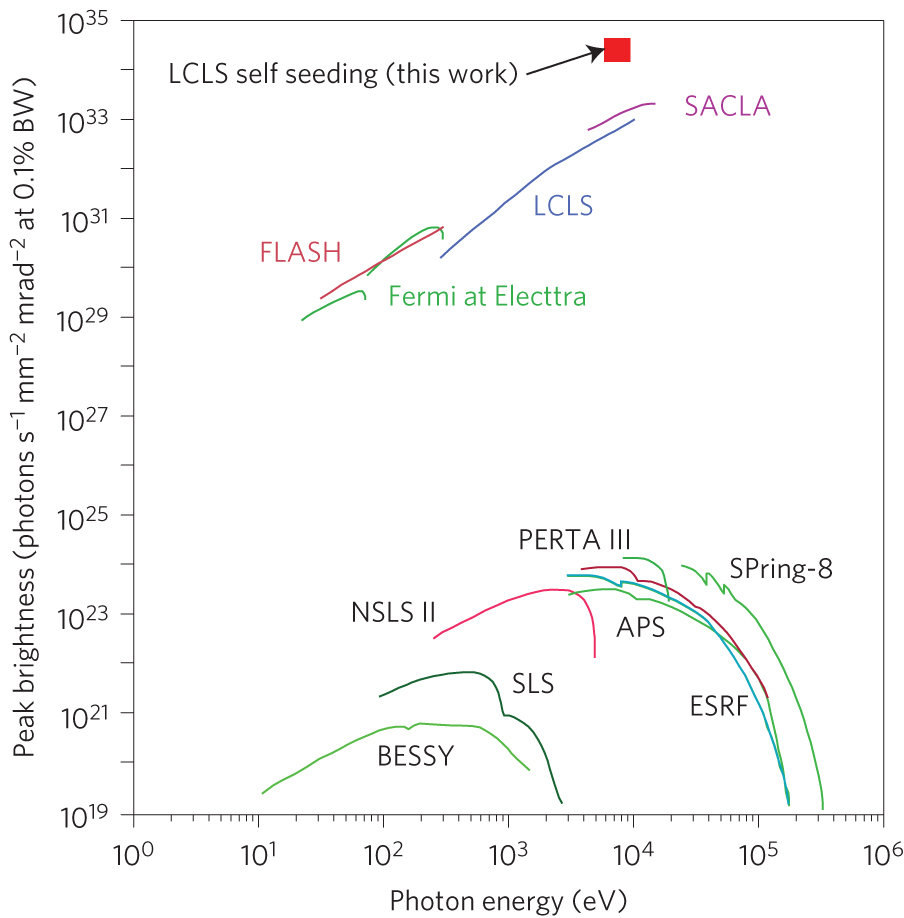
\includegraphics[width=0.49\textwidth]{images/spectral-brightness-fletcher-2015.jpg}
	\caption{caption. Right image from \citep{Fletcher-2015-NatPho}.}
	\label{fig:soft-xray-self-seeding}
\end{figure}
Free electron laser also have different operating modes than SASE. Particular interesting is the \textit{seeded} type of operation, where the FEL amplifies an initial seed of photons. The photons seed can be created through various processes. Here again, the wavelength of the photon seed is the critical parameter in determining which method to choose. For example, in the infra red (IR) to extreme ultra violet (XUV) regime, conventional lasers can be used to place the initial photons seed. However, due to the lack of lasers available at soft and hard X-rays wavelength regimes, the idea of \textit{self-seeding} gained traction. In self-seeding, an electron bunch is first send through a few undulator magnets to generate a few SASE photons, the electrons and photons are then separated using a magnetic chicane, which also neutralizes the microbunching in the electron bunch. The monochromator selects a small wavelength slice from the comparably broad SASE spectrum of the initial photons. The photons exiting the monochromator are considered the \textit{seed}. The seed and the electron bunch are overlapped again using the magnetic chicane and then send through more undulators. The seed generates now the microbuching, which is wavelength depended and thus a narrow wavelength band is amplified. Self-seeded beam operations have recently been demonstrated at LCLS. At hard X-rays, the Hard X-Ray Self-Seeding (HXRSS) instrument uses a diamond crystal to select a wavelength slice \citep{Amann-2012-NatPho}. At soft X-rays, the Soft X-ray Self Seeding (SXRSS) instrument uses a grating as dispersive element \citep{Ratner-2015-PRL}. A typical spectrum of a soft X-ray self-seeded beam can be seen in the left figure \ref{fig:soft-xray-self-seeding}. The characteristics of this spectrum are an intense peak at the selected wavelength regime on top of a broad SASE background. The background is an artifact of the amplification of some spontaneous emission events and can be suppressed by using fewer undulator magnets. Self-seeded beams have a significantly reduced pulse energy by an order of magnitude or so, depending on the exact beam parameters, as compared to SASE operations. However, in their main peak, self-seeded beams have a higher spectral brightness when compared to a SASE spectrum. SASE spectra usually have a broad spectral bandwidth with a $\Delta E$ of a few eV, comparing seeded beams with equation \ref{eq:spectral-brightness} to SASE beams the increase in spectral brightness using seeded beams is understandable and is illustrated in the right figure \ref{fig:soft-xray-self-seeding}. The peak intensity in a narrow spectral band makes seeded beams interesting for a variety of applications particular in condensed matter physics, where it is instrumental to excite with narrow bandwidth photons. Of course there are also applications in atomic and molecular physics, ranging from linear absorption spectroscopy \citep{Ferguson-2014-Unpublished}, to ultrafast photoemission spectroscopy on molecules \citep{Bucher-2014-Unpublished}, to non-linear stimulated Raman spectroscopy \citep{Kimberg-2016-FD}, to ultra-fast photoemission studies. Particular interesting for this work is the magnetic chicane from the SXRSS instrument that has been used as described in the next chapter.
\subsection{Novel X-ray pump–probe techniques}
%%%%%%%%%%%%%%%%%
%- Albertos pump-probe version\\
%- Agos two color pump probe version\\
%- Ratners and Agos seeded pump probe version\\
%- Use spectra from single-shot spectrometer
%%%%%%%%%%%%%%%%%%%%%%%%
In order to study X-ray induced methods using X-ray imaging and spectroscopy techniques, as it is discussed in the present work, two X-ray pulses are needed . Here, a pump pulse is used to induce dynamics in the sample system and a probe pulse is used to probe them at a certain time delay $\Delta t$. Pump--probe experiments are commonly used as they allow a precise study of dynamics. The pump pulse gives a very controllable starting point, i.e. time zero in the dynamic process, and the probe pulse can perform a measurement at a later time delay $\Delta t$. Sometimes pump and probe pulse are switched, which is indicated by a negative time delay $\Delta t$, often to verify time zero or to probe the system before any dynamics have occurred.\\
Creating two X-ray flashes to create a pump--probe experiment is a technical challenge and again this challenge is due to the lack of optics and the availability and size of X-ray SASE sources. In order to overcome this challenge, two methods have been proposed. Method one, mirror based beam-split and delay systems \citep{Castagna-2013-JPCS,Murphy-2012-SPIE} that split one pulse into a pump and probe beam and allow the delay of the latter. These systems typically are limited to short delay times, as the optics have to fit into existing setups and have a low transmission of X-rays over the mirrors. Method two, uses accelerator based schemes \citep{Lutman-2013-PRL,Marinelli-2015-NatComm} that manipulate electron bunches to create two X-ray pulses. Limitations arise depending on the scheme, e.g. limited pulse delay $\Delta t$ or pulse energy split through limited electron beam separation or length of magnetic chicane. Both methods have been demonstrated at LCLS and have found use to complement the more widely available optical laser pump-- X-ray probe methods particularly in the chemical sciences \cite{Picon-2016-NatComm,Ferguson-2016-SciAdv,Liekhus-Schmaltz-2015-NatComm}.\\
As the accelerator based X-ray pump -- X-ray probe method using a magnetic chicane has been used, let us describe these schemes in greater detail. Before we jump into the technical details, it is good to know that not only the aspect of creating a time delay $\Delta t$ between the pump and the probe pulse is important but also to create a difference in wavelength between these two pulses. Generally, this is of use to resonantly pump and off-resonance probe or vice versa. Equation \eqref{eqn:fundamental-wavelength} indicates which parameters can be tuned to create two pulses of different color. One, the undulator parameter K can be tuned to change the emitted wavelength, or two, the lorentz factor $\gamma$ can be different if there are two electron bunches. The undulator period $\lambda_{U}$ is fixed at LCLS.
\subsubsection{Undulator parameters $K_{1,2}$ based pump--probe scheme}
\begin{figure}
	\centering
		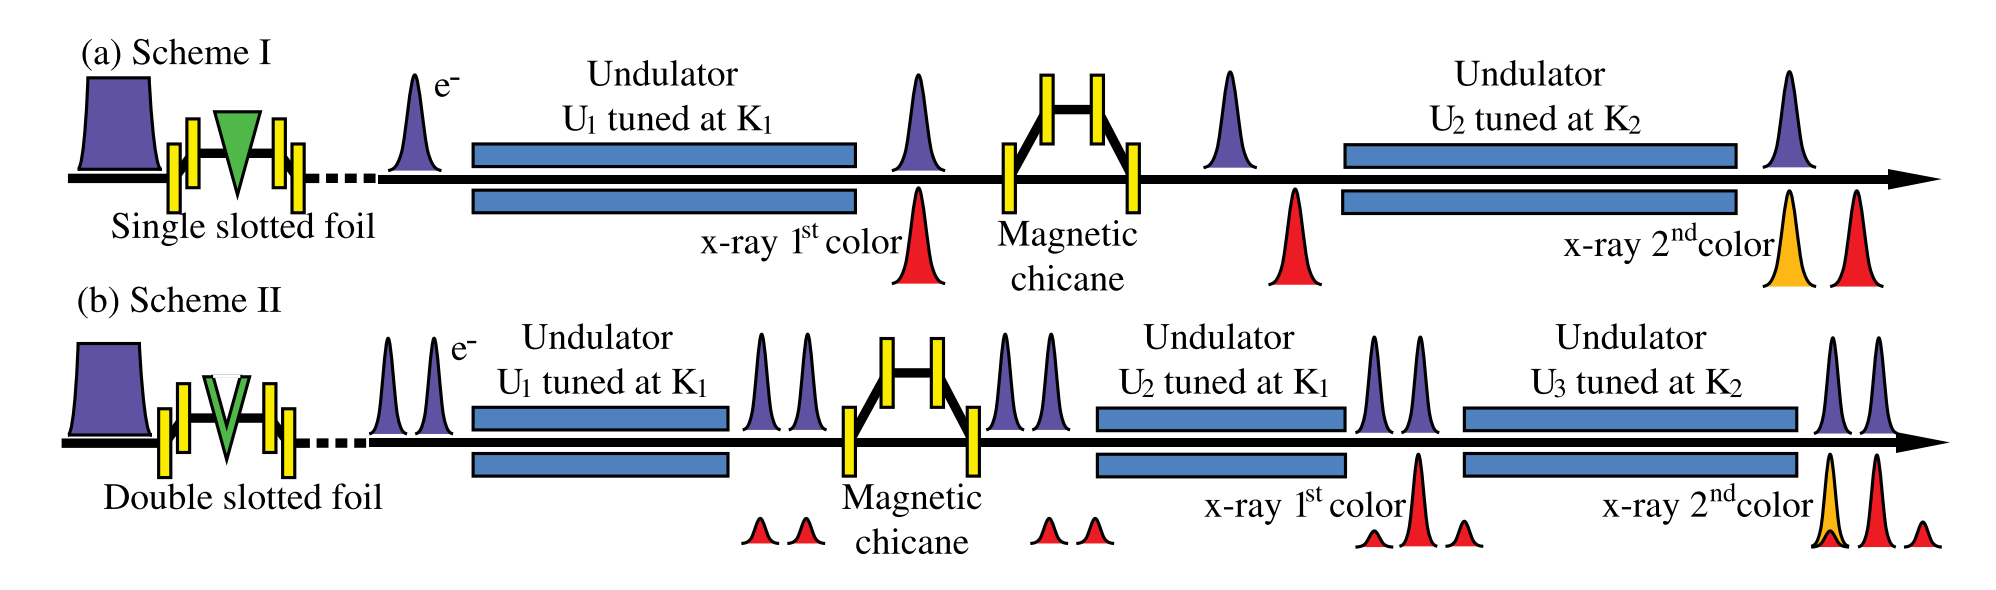
\includegraphics[width=1.00\textwidth]{images/Albertos-pump-probe-scheme.png}
	\caption{Schematic setup at LCLS of undulator parameter $K_{i}$ based pump--probe schemes. Scheme I creates one electron bunch using a single slotted foil and scheme II creates two electron bunches using a double slotted foil. The electron bunches emit radiation with a wavelength depending on $K_{i}$. A time delay $\Delta t$ between pulses is introduced using a magnetic chicane. Figure from \cite{Lutman-2013-PRL} reprinted with permission from APS.}
	\label{fig:Albertos-pump-probe-scheme}
\end{figure}
The first developed accelerator based pump--probe technique at LCLS \cite{Lutman-2013-PRL} uses a difference in undulator parameters $K_{1,2}$ to create two pulses of different wavelength, the time delay is introduced through a magnetic chicane and a schematic setup can be found in Figure \ref{fig:Albertos-pump-probe-scheme}.\\
In scheme I, one electron bunch is created through a single slotted foil\footnote{A single slotted foil or emittance-spoiling foil works comparable to a monochromator. It leaves a certain energy band of the electron bunch within the slot unspoiled and Coulomb scatters or spoils (compare to apertures) the rest. The 'dispersive' element is a magnetic chicane. By narrowing the electron beam one also reduces its pulse duration \cite{Emma-2004-PRL}.}  The use of the slotted foil enables control over the pulse duration. The electron bunch then travels through an undulator section $U_{1}$ tuned at strength parameter $K_{1}$ and is stimulated to lase but the process does not go into saturation to be able to reuse the electron bunch in the second undulator section. The time delay $\Delta t$ between the two pulses is introduced by a magnetic chicane. At LCLS, a dedicated chicane, e.g. from the soft X-ray self-seeding instrument, can reach up to
\begin{equation}
\Delta t_{max} = 800 fs.
\label{eq:alberto-delta-t-max}
\end{equation} The minimal time delay can be achieved by setting the deflection in the magnetic chicane to zero in which case
\begin{equation}
\Delta t_{min} = \frac{l}{v_{el\ drift}} - \frac{l}{c}\approx 0 fs,
\label{eq:alberto-delta-t-min}
\end{equation}
with $l\approx 4m$ being the length between undulator sections $U_{1}$ and $U_{2}$ and $c$ being the speed of light and $v_{el\ drift}$ being the drift velocity of the electron bunch. As the electron bunch travels close to the speed of light $t_{min}$ is typically on the tens of attosecond timescale. The timing jitter between the two light pulses using only one electron bunch comes solely from the magnetic chicane due to the magnetic field jitter and the electron beam energy jitter. The total contribution to the timing jitter is less than $0.4\%$ of the tim delay $\Delta t$ imposed by the chicane. Since the delay chicane does not contribute significantly to the delay $\Delta t$ a bigger factor is the velocity mismatch of the light pulse and the electron bunch. This mismatch can be estimated by
\begin{equation}
\Delta t_{beam\ mismatch}=\frac{N_{u} \lambda_{r}}{c},
\label{eq:alberto-beam-missmatch}
\end{equation}
with $N_{u}$ being the undulator periods. Given the parameters in study \cite{Lutman-2013-PRL}, $t_{beam\ mismatch}=3fs$ such that a partial overlap could be achieved. However, the magnetic chicane removes the microbunching from section $U_{1}$. In undulator section $U_{2}$ tuned to undulator strength parameter $K_{2}$ the electron bunch lases again and the process is able to saturate. The maximal color separation between the two pulses is $~ 1.9\%$ in relative difference between $K_{1}$ and $K_{2}$.\\
Scheme II uses a double slotted foil\footnote{A double slotted foil works as a single slotted foil but it leaves to parts of the electron beam unspoiled through the two slots.} to create two electron beams. The two beams have a longitudinal separation that translates into the time delay $\Delta t$. The electron bunches travel through a first set of undulators $U_{1}$ that creates two pulses of the same wavelength, due to the shortness of the section $U_{1}$ the lasing process does not saturate. The electron bunches are then delayed using a magnetic chicane such that the leading electron bunch overlaps with the trailing light pulse. This light pulse now functions as a seed for the leading electron bunch such that this pulse saturates in undulator section $U_{2}$. The electron bunches then travel through the magnets at $U_{3}$, where the trailing electron bunch creates a second saturated pulse, the leading electron bunch barely emits radiation in $U_{3}$ since its energy spread has become too large after lasing in $U_{2}$. Using this method, two saturated lasing pulses can be generated, however, temporal overlap cannot be achieved.
\subsubsection{Twin bunch or Lorentz factor $\gamma$ based pump--probe scheme}
\begin{figure}
	\centering
		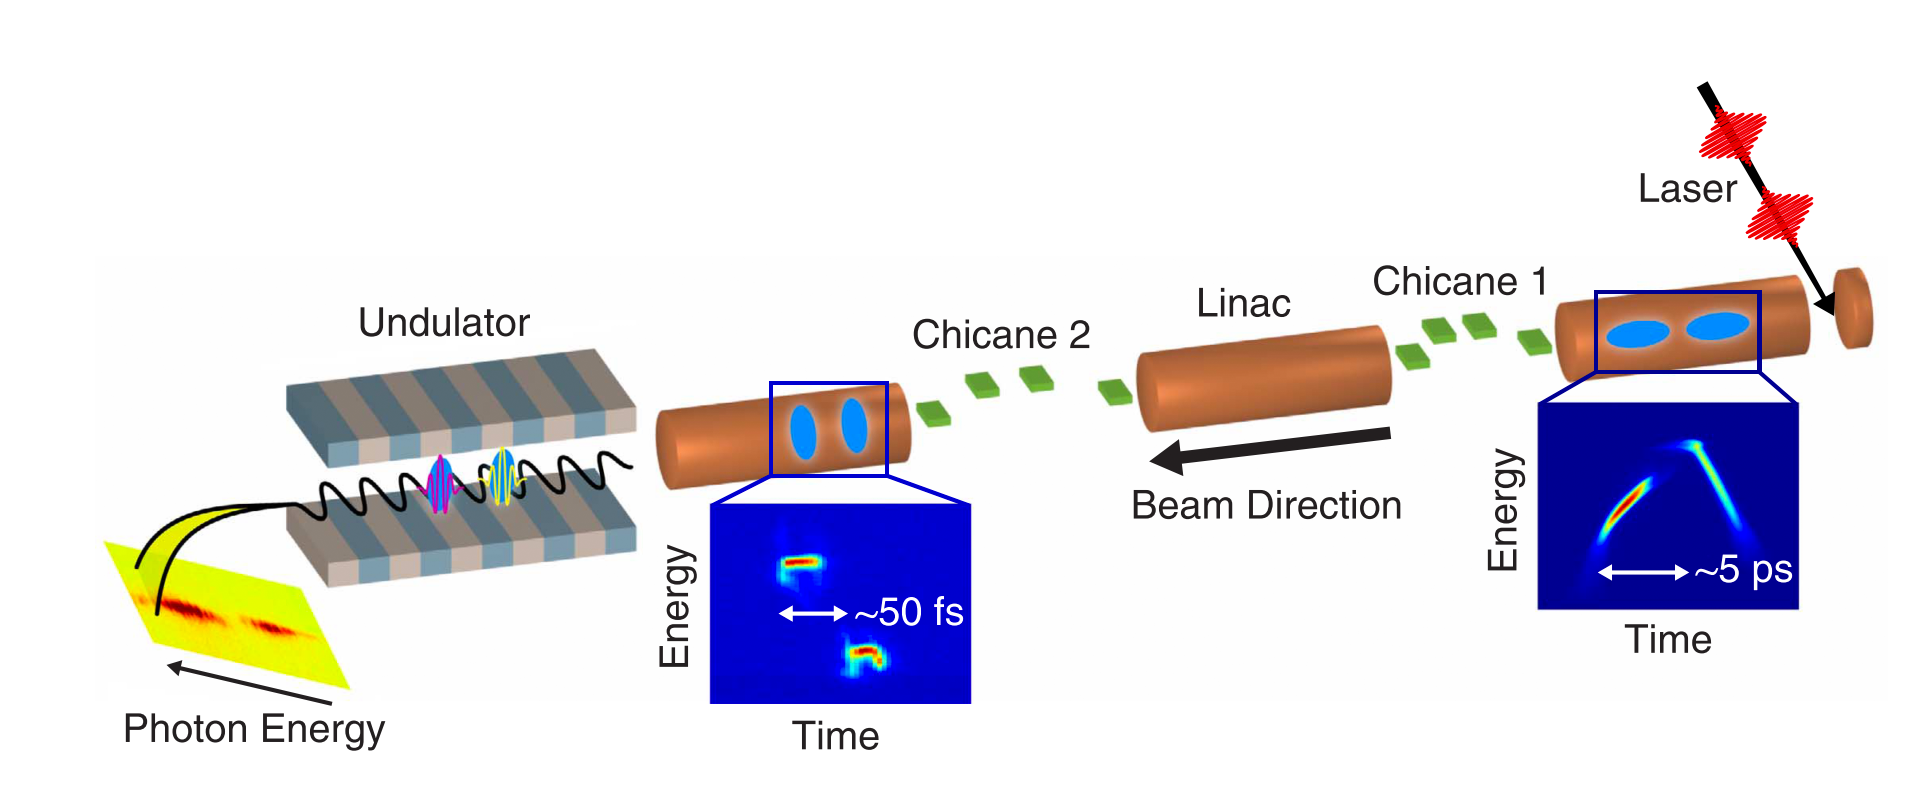
\includegraphics[width=1.00\textwidth]{images/Agos-pump-probe-scheme.png}
	\caption{Schematic setup of the two bunch, two color pump--probe setup at LCLS. Two laser pulses shot at a cathode create two electron bunches with a delay $\Delta t$ on the picosecond timescale. Two magnetic chicanes compress the bunches such that a delay $\Delta t$ on the up to the ten femtosecond timescale is achieved. Both pulses go through one undulator section and the SASE lasing process is saturated. The relative color separation is on the order of $1\%$.}
	\label{fig:Agos-pump-probe-scheme}
\end{figure}
The second developed accelerator-based pump-probe technique at LCLS \cite{Marinelli-2015-NatComm} uses two electron bunches of different energy. A schematic setup of this beam operation can be found in figure \ref{fig:Agos-pump-probe-scheme}.\\
The bunches are created through a double laser pulse that impinges on a photocathode. Initially, these two bunches have a time delay of a few picoseconds, however, two magnetic chicanes compress the electron bunches in the time and intensity domain such that a time delay on the ten femtosecond timescale is achieved. The electron bunches then travel through one undulator section and both pulses saturate in their lasing process. At $8.3k$ eV, both pulses combined can reach pulse energies of $1.2mJ$, the color separation is $100$ eV and the time separation ranges from $\Delta t_{min}=0fs$ to $\Delta t_{max}=100fs$. At hard X-rays, this method requires the pump pulse to have a higher photon energy than the probe pulse, although their respective intensities may vary. However, this method is not restricted to hard X-rays and can be utilized at soft X-rays. In the soft X-rays wavelength regime, where the above explained slotted spoiler foil can be used. This allows a further control to tune the time delay of the electron bunches, which enables scanning across each other.
%%%
\section{Rare gas clusters}\label{sec:cluster-theory}
%%%%%%%%
%- Why are rare gas clusters a suitable sample
%%%%%%%%
Rare gase clusters have been used as nanosample in this study and this chapter will explore this topic. Clusters have a long history to study light-matter interaction as their characteristics are well known \cite{Haberland-1994-Springer}. Generally speaking, clusters are an aggregation of atoms or molecules and vary in size. Their size can range from a few atoms to mesoscopic sizes such that one can classify a cluster as a bulk material. Clusters can form exotic materials that are interesting to study and can be well simulated through comparably simple computer models. Besides these testbed characteristics, the use of clusters has often practical purposes. They can be comparably easily generated and are typically easily tune able in size. Rare gas clusters are a subclass of clusters and they are bound by van der Waals forces and normally neutral-charged. Single van der Waals cluster typically form in an icosahedral\footnote{An icosahedron is a polyhedron with 20 faces, i.e. a dice with 20 faces.} shape when they are sufficiently small (up to nanometer sized) \cite{Miehle-1989-JCP} and have mostly a fcc-crystal\footnote{fcc is short for face-centered cubic. A very common crystal structure.} structure but exhibit also hcp-crystal\footnote{hcp stands for hexagonal close-packed and is also a crystal structure.} structures \cite{VanDeWaal-1993-JCP,Krainyukova-2006-TSF}. The creation of homogenous and heterogeneous rare gas clusters shall be the focus of the next few chapters.
\subsection{Creation of a homogenous cluster}
%%%%%%
%- the theory behind rare gas cluster creation.
%%%%%%
Rare gas clusters, for example xenon clusters, can be generated through a variety of ways. While there are many ways to explain the cluster formation process, a kinetic model \cite{Lippmann-1984-JCP} gives a very intuitive way in the microscopic processes. In this kinetic model, atoms and clusters grow through collisions. We can express these collisions mathematically through the following reaction formula
\begin{align}
A_{n}+A \rightleftharpoons A_{n+1}^{*},\quad n=1,2,...,\quad \mathrm{monomer\ collision,}
\intertext{where a body $A_{n}$ collides with a monomer $A$ and form a metastable state $A_{n+1}^{*}$ that will dissociate if not a subsequent collision deactivates it}
A_{n+1}^{*}+M\rightleftharpoons A_{n+1} + M,\quad \mathrm{activation/deactivation.}
\label{eq:early-cluster-growth}
\end{align}
$M$ is a chaperone that can be any kind of third body that removes energy from the system. Note that a chaperone $M$ can also activate the state again. The binding force behind rare-gas clusters is the Van der Waals force, hence they are called Van der Waals cluster sometimes.\\
While the early stage of the cluster growth is driven by the monomer addition, cluster-cluster coagulation start to dominate the later growth processes \cite{Zurek-1980-JCP,Soler-1982-PRL}. This is due to the quantitative increase in small clusters in the generation process that then start to collide, similar to above kinetic model. From empirical evidence, we know that clusters solely generated through monomer addition have a size distribution of an exponential decay, whereas larger clusters that grew through coagulation follow a log-normal distribution. So through coagulation, the density of smaller clusters (and monomers and dimers) decreases through to cluster-cluster coagulation and larger clusters are formed. The most probable size of a cluster, i.e. the maximum of the log-normal distribution, is given by the parameters of the supersonic jet setup, which is what we will discuss next.\\
\begin{figure}
	\centering
		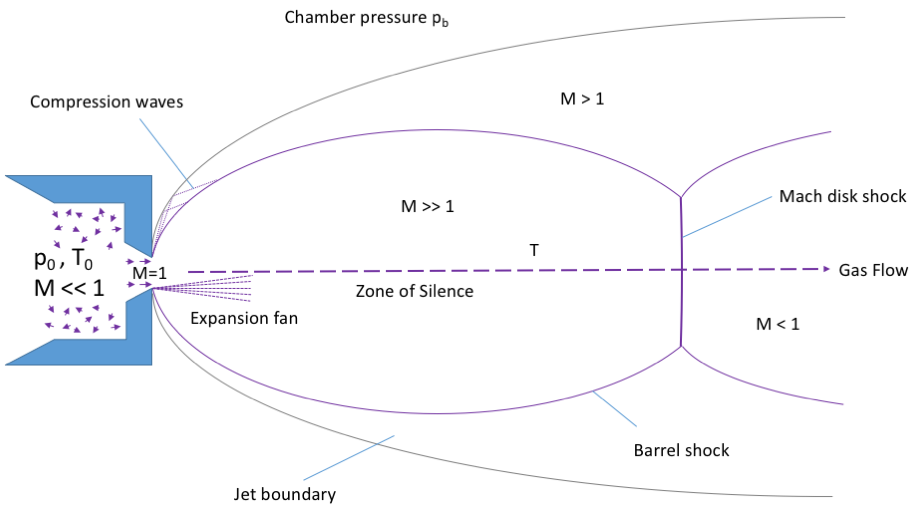
\includegraphics[width=1.00\textwidth]{images/freeJetExpansion.png}
	\caption{caption. After \cite{Miller-1988-Oxford}}
	\label{fig:freeJetExpansion}
\end{figure}
Supersonic jet setups typically store gas in a reservoir at a certain stagnation pressure $p_{0}$ and temperature $T_{0}$. The gas expands through a nozzle into a vacuum and figure \ref{fig:freeJetExpansion} shows a schematic drawing of this process. Typical values for $p_{0}$ are 10 bars, where the mean free path of the atoms is much smaller than the nozzle diameter D. This is why many collisions occur during the expansion in the nozzle and the above described kinetic theory explains the cluster formation. However, this holds not true in the supersonic molecular flow region, where no further cluster growth happens. To understand the expansion process in detail, we assume to work with an ideal gas and to describe the gas expansion itself, we further assume that no clusters are formed and that turbulence and effects of heat conduction are unimportant \cite{Yamada-2001-SciDir,Haberland-1994-Springer}.\\
To begin, the velocity distribution of the gas follows a Maxwell-Boltzman distribution with a mean velocity $\bar{v}$ that we can write down as
\begin{equation}
\bar{v}=\sqrt{\frac{2 k_{B}T_{0}}{m_{gas}}},
\label{eq:boltzman-mean-velo}
\end{equation}
with the Boltzman constant $k_{B}$ and the atomic mass of the gas $m_{gas}$. The movement direction of each atom is randomly orientated. Let us also define the enthalpy $H_{0}$ in the stagnation chamber
\begin{align}
H_{0}=c_{p} T_{0},
\intertext{with the specific heat $c_{p}$ for atoms}
c_{p}=\frac{5}{2}k_{B},
\label{eq:stagnation-enthalpy}
\end{align}
The expansion of the gas through the nozzle is driven by the pressure difference $p_{vac}/p_{0}$. In the nozzle, the (steady) gas flow becomes directed and the enthalpy $H_{0}$ is converted into kinetic energy $\frac{1}{2}m v^{2}$ and a rest enthalpy $H$. So, in the expansion process, we can use the conservation of energy, and equation \eqref{eq:stagnation-enthalpy} we can write down
\begin{equation}
H_{0}=H+\frac{1}{2}m_{gas} v^{2} = c_{p}T+\frac{1}{2}m_{gas}v^{2},
\label{eq:local-temperature}
\end{equation}
 with $T$ being the local temperature along the gas flow. To look at this in greater detail, let us define the Mach number $M$ as the ration of the stream velocity $v$ and the local speed of sound $c_{s}$
\begin{equation}
c_{s}=\sqrt{\frac{\gamma k_{B} T}{m_{gas}}}.
\label{eq:local-speed-of-sound}
\end{equation}
With the ratio of specific heats $\gamma = \frac{c_{p}}{c_{v}}$ at constant pressure and volume, they can be regarded as independent of temperature for atomic gases, we can rearrange equation \ref{eq:local-temperature} to 
\begin{equation}
T=T_{0}\left(1+\frac{1}{2}\left(\gamma - 1\right)M^{2}\right)^{-1}.
\label{eq:local-temperature-definition}
\end{equation}
Here the interplay between the Mach number $M^{2}$ and the local temperature $T$ give insight into the directed mass flow versus the remaining thermal energy in the system. As indicated the the figure \ref{fig:freeJetExpansion}, M increases dramatically along the expansion axis and that is due to decrease in speed of sound $c_{s}$ that is proportional to $\sqrt{T}$ as indicated in equation \eqref{eq:local-speed-of-sound}. Finally, this attribute has given the name to supersonic jets.\\
Let us describe the appearance of the jet stream (see figure \ref{fig:freeJetExpansion})next. Upon exiting the nozzle, the Mach number increases by a wide margin ($M>>1$), that means that the gas travels faster than information in this medium. Here, a \textit{zone of silence} is formed, where the gas flow is not influenced by other particles, thus uninterrupted. As the supersonic flow is exiting the nozzle it has to turn around the edge of the nozzle to further expand and the supersonic flow turns by actually creating smaller Mach waves. At the borders of the \textit{zone of silence}, $M$ decreases drastically resulting in dense regions that are called \textit{barrel shock} to the sides and \textit{Mach disk} downstream the gas flow. For an unhindered transport of the gas and clusters to the interaction region, the interaction region needs to be within the \textit{zone of silence}. We can express the distance from the nozzle to the Mach disk through
\begin{equation}
\frac{x_{MD}}{d}=0.67\left(\frac{p_{0}}{p_{b}}\right)^{\frac{1}{2}}.
\label{eq:distance-of-mach-disk}
\end{equation}
So the the competing stagnation pressure $p_{0}$ and the background pressure $p_{b}$ define the distance of the otherwise static parameters. Hence, $p_{b}$ needs to be low enough do drive the Mach disk downstream of the interaction region. By using skimmers and physically separating the jet expansion into separately pumped compartments, the background pressure $p_{b}$ can be reduced.\\
While we have described a cooling gas in the expansion process it should be noted that the clusters are comparably hot. Through the kinetic process described above, they are efficiently heated. The two processes to loose energy are, one, collisions with a chaperone $M$ that deactivates the cluster, or two, evaporation of monomers from the cluster. The evaporation process makes the temperature size-independent, after the clusters have reached a certain minimum size \cite{Farges-1981-SurfSci}. It is tedious and experimentally difficult to measure the temperature exactly but typically, the jet reaches temperatures of a few Kelvin and the cluster temperature is heavily dependent on their material, particular the dissociation energy. For this study relevant are mostly the temperature of Xenon cluster that is $~75K$\footnote{To put this temperature in perspective, krypton clusters are $~50K$ and argon cluster $~40K$ \cite{Farges-1981-SurfSci,Gspann-1986-Springer}. Note that in this study the cluster size was $\bar{N} > 800$, hence above the minum value to be size independent. For the evaporative cooling process to settle at a given temperature, a certain flight distance (in the cited study 6.5cm) should also be taken into account.} and the fact xenon clusters are solid because their melting temperature is higher\cite{Gspann-1986-Springer}. Follwing this same line of argumentation, helium clusters are liquid, which is why they are often called (helium-)droplets. If helium droplets are produced using a cryogenic jet even superfluid helium-droplets can be observed.\\
\begin{table}
	\centering
		\begin{tabular}{ | l | l | l | l | l | }
			\hline
			Helium & Neon & Argon & Krypton & Xenon \\ \hline
			3.85 & 185 & 1646 & 2980 & 5554 \\ \hline
		\end{tabular}
	\caption{Parameter K values for rare gases \cite{Schorb-2012-Thesis}.}
	\label{tab:k-parameter}
\end{table}
At the current point of the discussion, it should shine out that the average cluster size is very much depended on the gas type, stagnation temperature $T_{0}$, stagnation pressure $p_{0}$ and the nozzle type. Indeed, an empirically found scaling law named after Hagena \cite{Hagena-1972-JCP,Hagena-1981-SurfSci,Hagena-1987-ZeitschriftAMC}, can be written down as
\begin{equation}
\Gamma^{*} = K \cdot T_{0}^{0.25q-1.5} \cdot p_{0} \cdot d_{eq}^{q},
\label{eq:Hagena-parameter}
\end{equation}
with the gas specific parameter K that can be found in table \ref{tab:k-parameter} for some rare gases, the gas specific parameter $q$ that varies between 0.5 and 1 and is 0.85 for all rare-gases, and the equivalent nozzle opening $d_{eq}$ that is $d_{eq}=d$ for pinhole sources and for conical nozzles $d_{eq}$ reads
\begin{equation}
d_{eq} = d\frac{\tan\left(\Phi_{0}\right)}{\tan\left(\Phi\right)}
\label{eq:equivalent-nozzle-opening}
\end{equation}
with the half opening angle of the nozzle $\Phi$ and the half opening of the free gas expansion $\Phi_{0}$. The Hagena scaling parameter $\Gamma^{*}$ allows us to estimate the mean cluster size, i.e. amount of accumulated particles per cluster $<N>$, as follows
\begin{itemize}
	\item $\Gamma^{*} < 350$, no cluster formation observed.
	\item $350 < \Gamma^{*} < 1800$, in this region $<N>$ reads
		\begin{equation}
		<N> = 38.4 \left(\frac{\Gamma^{*}}{1000}\right)^{1.64}
		\label{eq:intermediate-hagena-scaling}
		\end{equation}
	\item $1800 < \Gamma^{*}$, in this region $<N>$ reads
		\begin{equation}
		<N> = 33.0 \left(\frac{\Gamma^{*}}{1000}\right)^{2.35}
		\label{eq:large-hagena-scaling}
		\end{equation}
\end{itemize}
Supersonic jets generally create clusters of different sizes. This size distribution is centered around $<N>$ and for solid rare gas clusters, this distribution is a log-normal distribution. The size distribution can be an experimental challenge, especially when size dependent effects are investigated. Free electron laser allow the determination of the size of a single cluster through a diffraction image and by measuring enough single clusters, one can reproduce size distributions as in figure \ref{Figure-size}. Historically, electron diffraction \cite{TBD} and interferometric approaches \cite{TBD} have been used to determine the size of clusters.\\
Experiments using supersonic jets for cluster generation are typically performed with pulsed valves to decrease cost and gas load in the overall system. Upon opening and closing of the valve, the gas density varies. This mostly affects the cluster size and one would expect to see smaller clusters. This remains true in the beginning of the pulse but in the \textit{afterpulse} one finds giant clusters that exceed the above described scaling laws \cite{Rupp-2014-JCP}.
%
%
%
%
%
\subsection{Creation of a heterogeneous cluster}
%%%%%%%%%%%%%%%%%
%- Heterogeneous clusters, e.g. He Xe\\
%- Do you have literature on that?
%%%%%%%%%%%%%%%%%
\begin{figure}
	\centering
		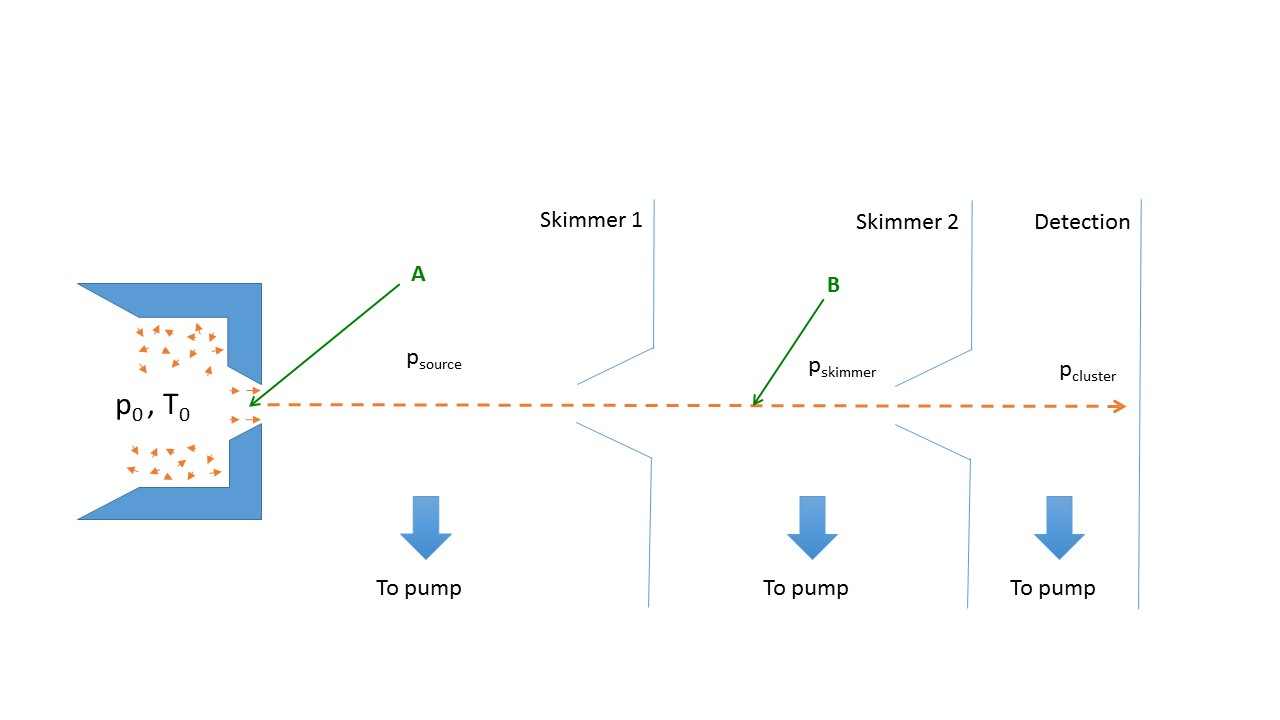
\includegraphics[width=1.00\textwidth]{images/pick-up.jpg}
	\caption{caption. After \cite{Gough-1985-JChemPhys,Haberland-1994-Springer}.}
	\label{fig:pickupPrinciple}
\end{figure}
The creation of heterogeneous clusters as they have been used in this study stands in the foreground of this chapter. One of the possibilities to create heterogeneous clusters is through the principle of picing-up atoms or molecules \cite{Gough-1985-JChemPhys,Haberland-1994-Springer}. Figure \ref{fig:pickupPrinciple} illustrates pickup regions that are typically used in an experiment. Mainly, there are two different pickup processes, one, monomers are added to the cluster in region A of figure \ref{fig:pickupPrinciple} that represents the nozzle of a supersonic source, or two, they can be picked up by a cluster in region B for example through an increase background pressure $p_{b2}$. If clusters pick up atoms or molecules in the nozzle region A, they can become part of the cluster formation and can be found inside of solid clusters. If atoms or molecules are picked up in region B, they stick to the surface of solid clusters but because the incoming cluster is so much larger and heavier than the colliding monomer the trajectory is not affected significantly. The collision does add energy to the cluster, which is why it will loose particles through evaporative cooling again. The loss of particles through evaporative cooling is proportional to the ratio in dissociation energies of the cluster and picked up material. Already pressures of $10^{-11}$ bars over a pickup length of a few centimeters can dope the cluster in significant form. At these low pressures, picking up atoms or molecules in region B requires less gas load on the system but is also less efficient than picking up in region B. To increase the pickup levels in region B, a gas cell can be used as much higher pressures can be achieved within the gas cell without putting too much load on the overall system.
%%%
\section{Introduction into X-ray scattering}\label{sec:scattering-theory}
%%%%%%%%%%%%%%%%%%%%%
%- Starting with Maxwell equations (this would be coming from the far end, I might be able to go into Guiniers formalism earlier. Depending on space.)\\
%- Mathematical model for electromagnetic wave\\
%- Kramers-Kronig relations\\
%- Mie scattering in a nutshell
%%%%%%%%%%%%%%%%%%%%%%%
This section will give  a brief introduction into the elastic scattering of X-rays with matter. The actual scattering process is very complex as it is an interplay of coherent, incoherent and elastic, inelastic processes. Fortunately, we can reduce the scattering description to its main process: The coherent and elastic scattering. In other words, we neglect Compton scattering (incoherent), any kind of absorption processes (inelastic) and effects form the scattering of multiple particles. We will then start this section by looking at the small angle scattering of atoms and continue on to extended objects such as clusters. The section is rounded off by an introduction to the inverse problem and basic algorithm ideas to overcome the issue of phase retrieval.
\subsection{Small angle X-ray scattering}
%%%%%%%%%%
%- Switch to Guiniers approximation and description\\
%- Work towards small angle scattering of small particles\\
%- Particular spheres\\
%- Discuss extreme positions
%%%%%%%%%%%
We can describe a linear polarized, electric field of a continuous electromagnetic wave via the following expression \cite{Als-Nielson-2011-JWS}
\begin{equation}
\vec{E}(\vec{r},t) = \vec{\epsilon} E_{0} e^{i \vec{k}\cdot\vec{r}},
\end{equation}
with $\vec{E}(\vec{r},t)$ being the electromagnetic field of the wave, the wave vector $\vec{k}$, the Cartesian coordinate vector $\vec{r}$, the complex amplitude if the electric field is then $E_{0}\exp^{i \vec{k}\cdot\vec{r}}$ and because of the polarization we use $\vec{\epsilon}$ such that $\vec{\epsilon}\cdot\vec{k}=\vec{k}\cdot\vec{E}=\vec{k}\cdot\vec{H}=0$. If this wave encounters an electron, we can describe the scattering semi-classical by imagining how the electric field of the electron starts to oscillate once it sees an incoming electric wave. The electron then functions as a dipole antenna eventually radiating the wave into a certain solid angle $\Delta \Omega$. Through a relative comparison, of the incoming intensity and the scattered intensity, we can phenomenological establish the differential cross-section as
\begin{align}
\left(\frac{d\sigma}{d\Omega}\right)&=\frac{\left(\text{Number of X-rays scattered per second into $\Delta \Omega$}\right)}{\left(\text{Incident flux}\right)\left(\Delta\Omega\right)}=\frac{I_{sc}}{\left(I_{0}/A_{0}\right)\Delta\Omega},
\label{eq:scattering-crosssection}
\end{align}
with $A_{0}$ being the covered area of the incident beam. And depending on the polarization of the incident beam we can reduce equation \ref{eq:scattering-crosssection} to
\begin{align}
\left(\frac{d\sigma}{d\Omega}\right)&=r_{0}^{2}P,
\intertext{with the classical electron radius $r_{0}=2.82\ 10^{-5}$ \AA and the polarization factor P}
P&=\begin{cases}
1& \text{vertical scattering plane},\\
\cos^{2}\left(\Psi\right)&\text{horizontal scattering plane},\\
\frac{1}{2}\left(1+\cos^{2}\left(\Psi\right)\right)& \text{unpolarized source.}
\end{cases}
\end{align}
We can now move on and use this knowledge for atoms, where we have Z electrons. To describe electrons in an atom, let us proceed purely classical by introducing the electron density $\rho_{e}\left(\vec{r}\right)$ that describes the distribution of electron in an atom on average. Now, figure \ref{fig:X-ray-scattering} illustrates the scattering process in one atom. An incident beam with wave number $\vec{k}$ is elasticity scattered at a point $\vec{r}$ into a wave with $\vec{k}'$ such that $\left|\vec{k}\right|=\left|\vec{k}'\right|$. In this wave picture, the scattering process must be seen as a superposition of waves and it is particular illustrated how the wave scattered at the origin of the atom is scattered as well. As both waves are scattered at different points, they have an optical path difference $2 \delta$. This difference in path length results in a phase difference to each other and eventually leads to interference between the waves. So, we can describe the phase difference $\Delta \Phi\left(\vec{r}\right)$ of the waves scattered at $\vec{r}$ and the origin by
\begin{equation}
\Delta \Phi\left(\vec{r}\right) = \left(\vec{k}-\vec{k}'\right)\cdot \vec{r} = \vec{Q} \cdot r,
\label{eq:phase-difference}
\end{equation}
with $\vec{Q}$ being denoted as the \textit{wave-vector transfer}. Through trigonometry, we can then establish the more common denotation of the wave-vector $\vec{Q}$
\begin{equation}
\vec{Q}=2 \left|\vec{k}\right| \sin\left(\Theta\right)=\frac{4 \pi}{\lambda}\sin\left(\Theta\right),
\label{eq:Q-scattering-angle}
\end{equation}
with the wavelength of the light $\lambda$ and the scattering angle $\Theta$.\\
A volume element $d\vec{r}$ at $\vec{r}$ will now scatter depending on its electron density, namely by $-r_{0}\rho\left(\vec{r}\right)d\vec{r}$. At scattering angle 0, i.e. $\vec{Q}=0$ the atomic form factor $f^{0}$ is
\begin{equation}
f^{0}\left(\vec{Q}\rightarrow 0\right)=Z,
\label{eq:transform-number-of-particles}
\end{equation}
as all scatter are in phase. As we increase the scattering angle $\Theta$, the phase difference $\Delta \Phi\left(\vec{r}\right)$ leads to interference and we can describe this via a phase factor $e^{i \vec{Q}\cdot \vec{r}}$, hence $f^{0}\left(\vec{Q}\rightarrow\infty\right)=0$. If we integrate over the total scattering length, we can then write down
\begin{equation}
-r_{0} f^{0}\left(\vec{Q}\right)=-r_{0}\int\rho_{e}\left(\vec{r}\right)e^{i \vec{Q}\cdot \vec{r}}d\vec{r}.
\label{eq:scattering-integral}
\end{equation}
\begin{figure}
	\centering
		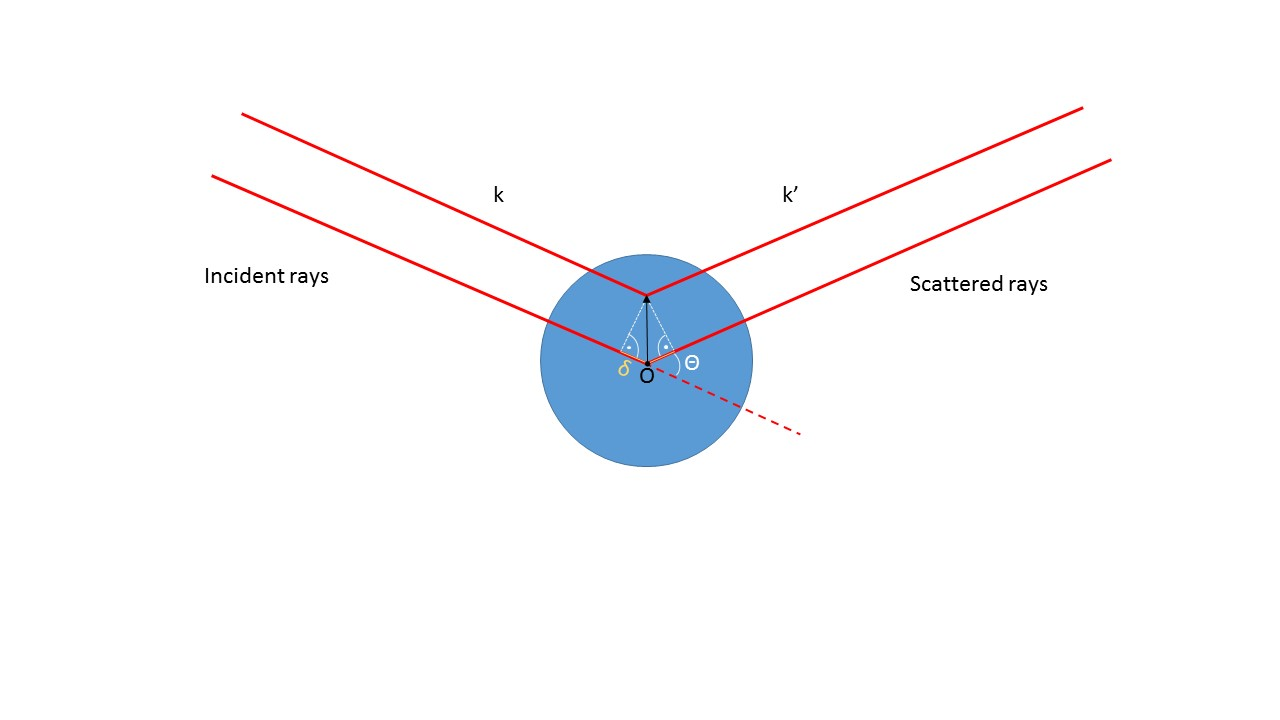
\includegraphics[width=1.00\textwidth]{images/X-ray-scattering.jpg}
	\caption{caption. After \cite{Als-Nielson-2011-JWS,Guinier-1955-JWS}.}
	\label{fig:X-ray-scattering}
\end{figure}
The atomic form factor can hence be seen as a Fourier transform of the classical electron density of an atom. To make it more clear, (X-ray) diffraction projects an image of the atom in reciprocal space.\\
Let us continue with the scattering of a molecule or cluster. We can label the atoms in such a particle by
\begin{equation}
F^{cluster}\left(\vec{Q}\right)=\sum_{j}f_{j}^{0}\left(\vec{Q}\right)e^{i \vec{Q}\cdot \vec{r}},
\label{eq:scattering-factor-cluster}
\end{equation}
with the atomic scattering factors $f_{j}^{0}\left(\vec{Q}\right)$ for the $j$'th atom and call $-r_{0} F^{cluster}$ the scattering length of a cluster. Strictly speaking, $F^{cluster}\left(\vec{Q}\right)$ is angle depended. However, in the angular range of $\vec{Q}$, where $F^{cluster}\left(\vec{Q}\right)$ is not 0, $f_{j}^{Q}\left(0\right)$ can be considered constant \citep[see][p. 6-7]{Guinier-1955-JWS}. In human hemoglobin, the range in which the molecule scattering length is not 0, the carbon atomic scattering factors change less than $0.4$\%. It is therefore most convenient to describe the scattering of extended objects via a continuous electron density, where certain volume elements $d\vec{r}$ scatter proportional to their electron density $\rho_{e}\left(\vec{r}\right)$. We can therefore go forward with a continuous description of extended objects using a generalized electron density $\rho\left(\vec{r}\right)$.\\
Let us summarize this briefly by recalling from optics in general that a lens is performing an inverse Fourier transformation to project the scattering from an object as a realspace image. Through expressing the probability of presence of an electron in the scattering process through a general electron density $\rho\left(\vec{r}\right)$ of an object. The reason why this is important is that free electron laser are the first light-sources to have enough photons in just one light pulse to generate a snapshot of a nanometer-sized particle, e.g. a biomolecule, in just one shot. The total scattered intensity $I\left(\vec{Q}\right)$ in a measurement is
\begin{equation}
I\left(\vec{Q}\right)=\left|A\right|^{2}=I_{0}\left|F^{0}\left(\vec{Q}\right)\right|^{2},
\label{eq:scattered-intensity}
\end{equation}
with the incident beam intensity $I_{0}$, the (complex) amplitude $A$\index{amplitude!complex} and
\begin{equation}
F^{0}=\int \rho\left(\vec{r}\right) e^{i \vec{Q}\cdot r}d\vec{r}.
\label{eq:scattering-factor-general}
\end{equation}
Clusters can be considered as spherical symmetric and if we assume such an electron density density $\rho\left(\vec{r}=\{0,..,R\}\right)=1$ of a particle with radius R, we solve the integral in equation \eqref{eq:scattering-factor-general} through transforming into spherical coordinates
\begin{align}
F_{Sphere}^{0}\left(\vec{Q}\right) &= \int_{0}^{\pi}\int_{0}^{2\pi}\int_{0}^{R} r^{2}  sin\left(\Theta\right) e^{i Q r \cos\left(\Theta\right)} dr d\Theta d\Phi\\
&=\frac{\sin\left(\vec{Q} R\right)-\vec{Q} R\cos\left(\vec{Q} R\right)}{\vec{Q}^{3} R^{3}}=\frac{J_{1}\left(\vec{Q}R\right)}{\vec{Q}R},
\label{eq:scattering from sphere}
\end{align}
with $J_{1}$ being the Bessel function of first kind. Formula \eqref{eq:scattering from sphere} can be easily abused to determine the size of a spherical particle using the local minima in the diffraction pattern.\\
The process of measuring the scattered light, e.g. through a detector, one merely measures the modulo of an amplitude $\left|A\right|^{2}$, which eliminates the phase factor $e^{i\Delta\Phi\left(\vec{r}\right)}\cdot e^{-i\Delta\Phi\left(\vec{r}\right)}=1$. In order to reconstruct the object that scattered in realspace, e.g. to understand its shape or to study its function, we need to recover this phase information. We will discuss this briefly in the next section.
%
%
%\subsection{X-ray diffraction}
%- I wonder if I should include this to talk about 'what happens on faster timescales' using Ken's work.
\subsection{The inverse problem: Phase retrieval}
%%%%%%%%%%%%%%
%- Introduce some aspects from phase retrieval algorithms.
%%%%%%%%%%%%%%
\begin{figure}
	\centering
		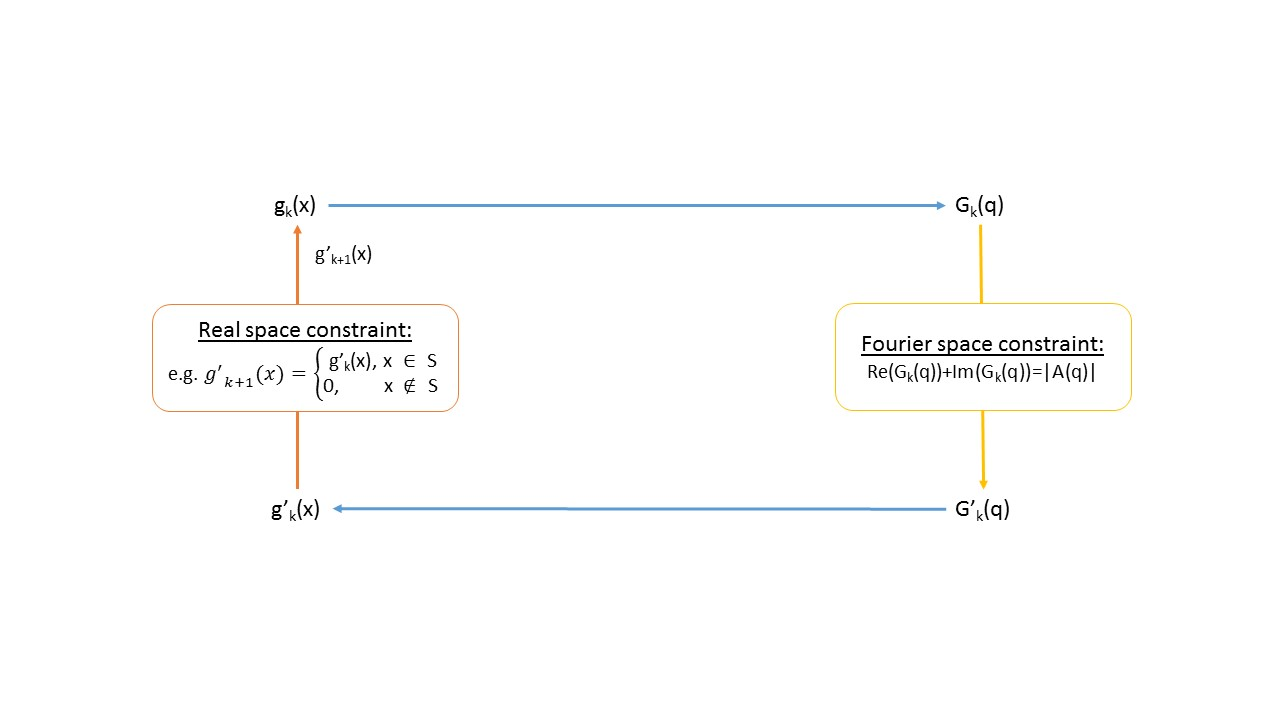
\includegraphics[width=1.00\textwidth]{images/phase-retrieval-algorithm.jpg}
	\caption{caption}
	\label{fig:phase-retrieval-algorithm}
\end{figure}
The loss of the phase in the scattering process results ultimately in a sign problem. The scattered intensity $I\left(\vec{Q}\right)$ is proportional to the form factors $\left|f^{0}\right|^{2}$. To recover the phase and thus reconstruct the particle iterative algorithms have been developed \cite{Fienup-1982-AO}. Figure \ref{fig:phase-retrieval-algorithm} illustrates such an iterative algorithm, where the image of an object $g_{k}\left(x\right)$ is Fourier transformed to reciprocal space $G_{k}\left(x\right)$ and then back again resulting in $g_{k+1}(x)$, while sufficing certain criteria.\\
The constraints are rather strict define in the reciprocal space as they have to reproduce the actual measurement $I=A\cdot A^{*}$. The constraints that need to be met can be chosen more freely. Generally, the recovered object should be physical, i.e. consist of positive values or should be of a certain (known) size. In simplified terms, one can introduce a support structure $S$ that meets the physical criterion and can therefore be used to, for example, zero outling values. Throughout the iterations the functions $g_{k}(x)$ evolve and eventually converge into a solution. If one uses the above criterion, one can show that the error between the reconstructions and the actual measurement continuously reduces, which is why it is commonly referred to as error-reduction algorithm \cite{Fienup-1978-OL}.\\
It should be noted that there is a great variety of manipulations that can be done upon not fulfilling a realspace constraint and although their function is fairly similar there is a great variety of algorithms. Worth mentioning is the hybrid input-output (hio) \cite{Fienup-1978-OL} and the relaxed averaged alternating reflection (RAAR) \cite{Luke-2005-IP}.
\section{Light-matter interaction}
Photons can also be absorbed by atoms in which case an electron get either excited to another state or ionized. At X-ray wavelengths matter typically gets ionized in the inner shells. Upon absorption a cascade of relaxation processes begins and the now ionized atom finds the new most energetic favorable state. These processes are particularly depended on the wavelength of the incident photons but also the type of atom. This chapter is devoted to these processes and particular the absorption process is described in section \ref{sec:absorption} and the relaxation processes in \ref{sec:relaxation}.
\subsection{Ionization of matter}\label{sec:absorption}
Let us quickly remember the atomic scattering factor $f^{0}\left(\vec{Q}\right)$, which we were able to introduce by neglecting a variety of (wavelength depended) effects through Fourier transforming the electron density of an atom. If we imagine (soft) X-rays approaching an atom classically, we can compare it to the analogon to a forced harmonic oscillator, where an electric field drives a (bound) electron. As a result, the phase velocity of light $v_{\text{phase}}$ is reduced to the speed of light in vacuum $c$ through interacting with electrons. Also if the the energy of the photons is higher than binding energies of electrons in the atom then also a probability for dissipation/absorption exists \citep{Als-Nielson-2011-JWS,Attwood-2007-CUP}. These two effects are connected to the atomic scattering factors $f^{0}\left(\vec{Q}\right)$ and are called dispersion corrections. Let us write down these two corrections
\begin{equation}
f\left(\vec{Q},\hbar\omega\right)=f^{0}\left(Q\right)+f'\left(\hbar\omega\right)+i f''\left(\hbar\omega\right),
\label{eq:scattering-factor-dispersion-corr}
\end{equation}
where $f'\left(\hbar\omega\right)$ corrects for the phase velocity and the wave amplitude correction/absorption $f''\left(\hbar\omega\right)$. In the limit of high photon energies $\hbar \omega$ the electrons can be largely seen as free, as the binding energies become a little factor, and $f'\left(\hbar\omega\right)\rightarrow 0$ and $f''\left(\hbar\omega\right)\rightarrow 0$. As the photon energies $\hbar \omega$ are closer to the atomic level, which is the case at soft X-rays for many materials, $f'\left(\hbar\omega\right)$ and $f''\left(\hbar\omega\right)$ can become large factors. Note particularly that these corrections only apply to the forward scattering, where $\vec{Q}=\Theta=0$.\\
We shall not derive this relation in its full extend that can be read in \citep[see][p. 55ff]{Attwood-2007-CUP}, but we shall compare the equation for the complex refractive index $n\left(\omega\right)$
\begin{equation}
n\equiv \frac{c}{v_{\text{phase}}}=1-\delta+i\beta
\label{eq:complex-refractive-index}
\end{equation}
to these arguments, as a wave propagating in a medium along the axis $z$ can then be written as
\begin{equation}
e^{i n k z}= \underbrace{e^{i \left(1-\delta\right)k z}}_{\text{phase shift}}\underbrace{e^{-\beta z}}_{absorption}.
\label{eq:wave-in-medium}
\end{equation}
And indeed, we are allowed to define this dispersion relation through the atomic scattering factors \citep{Als-Nielson-2011-JWS}
\begin{equation}
n\equiv 1- \frac{2\pi \rho_{atom}r_{0}}{k^{2}}\left(f^{0}\left(\vec{Q}=0\right)+f'\left(\hbar\omega\right)+f''\left(\hbar\omega\right)\right),
\label{eq:eq:complex-refractive-index-atomic-factors}
\end{equation}
with the atomic number density $\rho_{at}$ and we identify
\begin{align}
\delta &= \frac{2 \pi \rho_{atom} r_{0}}{k^{2}}\left(f^{0}\left(\vec{Q}=0\right)+f'\left(\hbar\omega\right)\right),\quad \text{and}\\
\beta &= - \left(\frac{2\pi \rho_{atom}r_{0}}{k^{2}}\right)f''\left(\hbar\omega\right).
\label{eq:delta-and-beta}
\end{align}
We have already established that $f''\left(\hbar\omega\right)$ reduces the amplitude of the incoming wave through absorption. Thus, using the absorption part of equation \eqref{eq:wave-in-medium}, we can rewrite $f''\left(\hbar\omega\right)$ in terms of an absorption cross section $\sigma_{a}$
\begin{equation}
f''\left(\hbar\omega\right)=-\left(\frac{k}{4\pi r_{0}}\right)\sigma_{a}.
\label{eq:f-2-definition}
\end{equation}
\begin{figure}
	\centering
		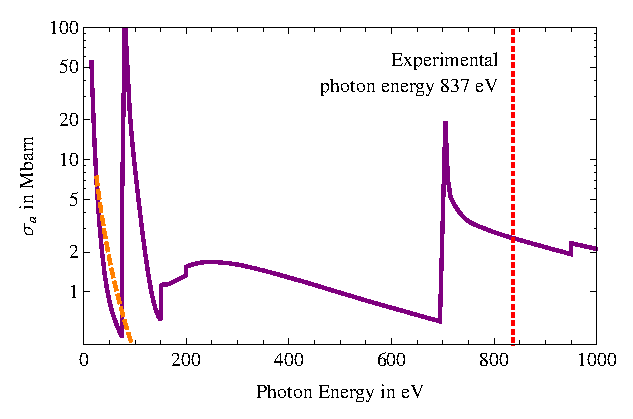
\includegraphics[width=1.00\textwidth]{images/photoionization.eps}
	\caption{caption. Data from \citep{Elettra-2016-Website,Yeh-1985-AtmDat,Yeh-1993-GBSP}}
	\label{fig:photoionization}
\end{figure}
Figure \ref{fig:photoionization} shows the absorption cross-sections $\sigma_{a}$ for xenon, helium and indicates the photon energy the experiment described in the next chapters has been conducted with.


%
%
%
%
%
\subsection{Charge migration}\label{sec:relaxation}
%%%
\section{Ionization of clusters in intense X-ray pulses}
- Short introduction coming from inelastic scattering
\subsection{Formation of nanoplasma}
- Step by step explanation on the formation of a nanoplasma
\subsection{Tampered layers to inhibit the nanoplasma expansion}
- Step by step explanation on the formation of the nanoplasma, pointing out the differences between tampered and pristine clusters.